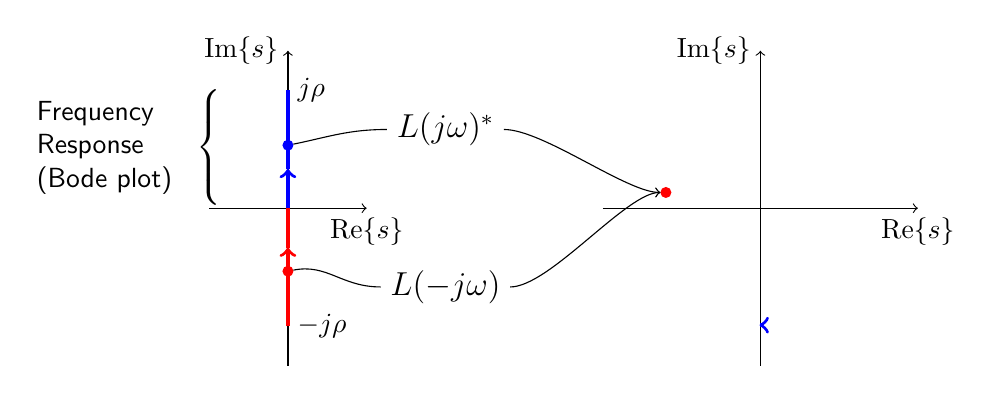
\begin{tikzpicture}[
sysblock/.style={draw,rectangle,inner sep=6pt,minimum width=1.25cm,minimum height=1.0cm,very thick},
summer/.style={circle,draw,very thick}]

\draw[->] (-4,-2) -- ++(0,4) node[left] {Im$\{s\}$};
\draw[->] (-5,0) -- ++(2,0) node[below] {Re$\{s\}$};
\draw[->,very thick,color=blue] (-4,0) -- (-4,.5); 
\draw[very thick,color=blue] (-4,.5) -- (-4,1.5);
\draw[->,very thick,color=red] (-4,-1.5) -- (-4,-.5); 
\draw[very thick,color=red] (-4,-.5) -- (-4,0); 

\draw (-4,1.5) node {\rule{4pt}{0pt}} node[right] {$j\rho$};
\draw (-4,-1.5) node {\rule{4pt}{0pt}} node[right] {$-j\rho$};
%\draw (-4,0) node[circle,fill,inner sep=0pt,outer sep=0pt,color=green] {\rule{4pt}{0pt}};
\draw (-4,.8) node[circle,fill,inner sep=0pt,outer sep=0pt,color=blue] (p1) {\rule{4pt}{0pt}};
\draw (-4,-.8) node[circle,fill,inner sep=0pt,outer sep=0pt,color=red] (p3) {\rule{4pt}{0pt}};
\draw (0.8,0.2) node[circle,fill,inner sep=0pt,outer sep=0pt,color=red] (p2) {\rule{4pt}{0pt}};
\draw (-2,1) node (L) {\large $L(j\omega)^{*}$};
\draw (-2,-1) node (L2) {\large $L(-j\omega)$};
\draw (p1) .. controls ++(.5,.1) and ++(-.5,0) .. (L.180);
\draw[->] (L.0) .. controls ++(.5,0) and ++(-.5,0) .. (p2);

\draw (p3) .. controls ++(.5,.1) and ++(-.5,0) .. (L2.180);
\draw[->] (L2.0) .. controls ++(.5,0) and ++(-.5,0) .. (p2);

\draw (-6,.8) node {\begin{minipage}{.75in}\textsf{Frequency Response (Bode plot)}\end{minipage} $\left\{\rule{0in}{.35in}\right.$};

\draw[->] (0,0) -- ++(4,0) node[below] {Re$\{s\}$};
\draw[->] (2,-2) -- ++(0,4) node[left] {Im$\{s\}$};

\draw[color=blue,very thick] plot[smooth] file {figures/nyquistmapping1.table};
\draw[color=red,very thick] plot[smooth] file {figures/nyquistmapping2.table};
\draw[->,very thick,color=blue] (2,-1.485) -- ++(-.01,0);

%\draw (2,.026) node[circle,fill,inner sep=0pt,outer sep=0pt,color=yellow] {\rule{4pt}{0pt}} ;
%\draw (3.4,0) node[circle,fill,inner sep=0pt,outer sep=0pt,color=green] {\rule{4pt}{0pt}};




\end{tikzpicture}